\documentclass[12pt,letterpaper]{article}
\usepackage{fullpage}
\usepackage[top=2cm, bottom=4.5cm, left=2.5cm, right=2.5cm]{geometry}
\usepackage{amsmath,amsthm,amsfonts,amssymb,amscd}
\usepackage{lastpage}
\usepackage{enumerate}
\usepackage{fancyhdr}
\usepackage{mathrsfs}
\usepackage{xcolor}
\usepackage{graphicx}
\usepackage{listings}
\usepackage{hyperref}
\usepackage{bm}

\hypersetup{%
  colorlinks=true,
  linkcolor=blue,
  linkbordercolor={0 0 1}
}
 
\renewcommand\lstlistingname{Algorithm}
\renewcommand\lstlistlistingname{Algorithms}
\def\lstlistingautorefname{Alg.}

\lstdefinestyle{Python}{
    language        = Python,
    frame           = lines, 
    basicstyle      = \footnotesize,
    keywordstyle    = \color{blue},
    stringstyle     = \color{green},
    commentstyle    = \color{red}\ttfamily
}

\setlength{\parindent}{0.0in}
\setlength{\parskip}{0.05in}

% Edit these as appropriate
\newcommand\course{VisNav}
\newcommand\hwnumber{1}                  % <-- homework number
\newcommand\NetIDa{Meng Liu}           % <-- NetID of person #1
%\newcommand\NetIDb{netid12038}           % <-- NetID of person #2 (Comment this line out for problem sets)

\pagestyle{fancyplain}
\headheight 35pt
\lhead{\NetIDa}
%\lhead{\NetIDa\\\NetIDb}                 % <-- Comment this line out for problem sets (make sure you are person #1)
\chead{\textbf{\Large Exercise \hwnumber}}
\rhead{\course \\ \today}
\lfoot{}
\cfoot{}
\rfoot{\small\thepage}
\headsep 1.5em

\begin{document}

\section*{Exercise 1: What is SLAM}

\begin{enumerate}
	\item The robot needs the map to localize itself in a scene. The map can also give human operators a visualization of the working environment of the robot.
	\item We can use SLAM in indoor mobile navigation applications, where the localization applications such as GPS can't work properly. 
	\item The history of SLAM can be separated into two parts:
	\begin{enumerate}
		\item Classical age (1986-2004) used a probabilistic point of view, and pointed out the problem of efficiency and robust data association.
		\item Algorithmic-analysis age (2004-2015) enriched the fundamental studies and practical utilities of SLAM (e.g. open-source libraries).
	\end{enumerate} 

\end{enumerate}

%---------------------------------------------------------------------------
\section*{Exercise 2: git, cmake, gcc, merge-requests}
\begin{enumerate}
	\item Give the variable \textbf{CMAKE\_MODULE\_PATH} a string, which contains the path to folder \textit{cmake\_modules}.
	\item Globally enable particular C++ standard for building the project, in this case, C++ 11; and disable C++ extensions.
	\item
	\begin{enumerate}
		\item Don't use optimization in debug build (fast compilation time), but get the debugging information; intialize all entries of newly constructed matrices and arrays to NaN; builds executable with debugging symbols for Clang debugger.
		\item Default build the release with debug info (higher level of optimization, slower compile-time); intialize all entries of newly constructed matrices and arrays to NaN; builds executable with debugging symbols for Clang debugger.
		\item Use optimization in release build; turn on lots of compiler warning flags; disable assertions; disable the limit of template instantiation backtrace
	\end{enumerate}
	\item Add an executable target called ``calibration" to be built from the source file \textit{calibration.cpp}. Then specify libraries (ceres, pangolin, and Threading Building Blocks) to be used when linking the target ``calibration".
\end{enumerate}

%---------------------------------------------------------------------------
\section*{Exercise 3: $SO(3)$ and $SE(3)$ Lie groups}
Assume $\phi = \theta \bm{a}$,
\begin{figure}[hbt]
  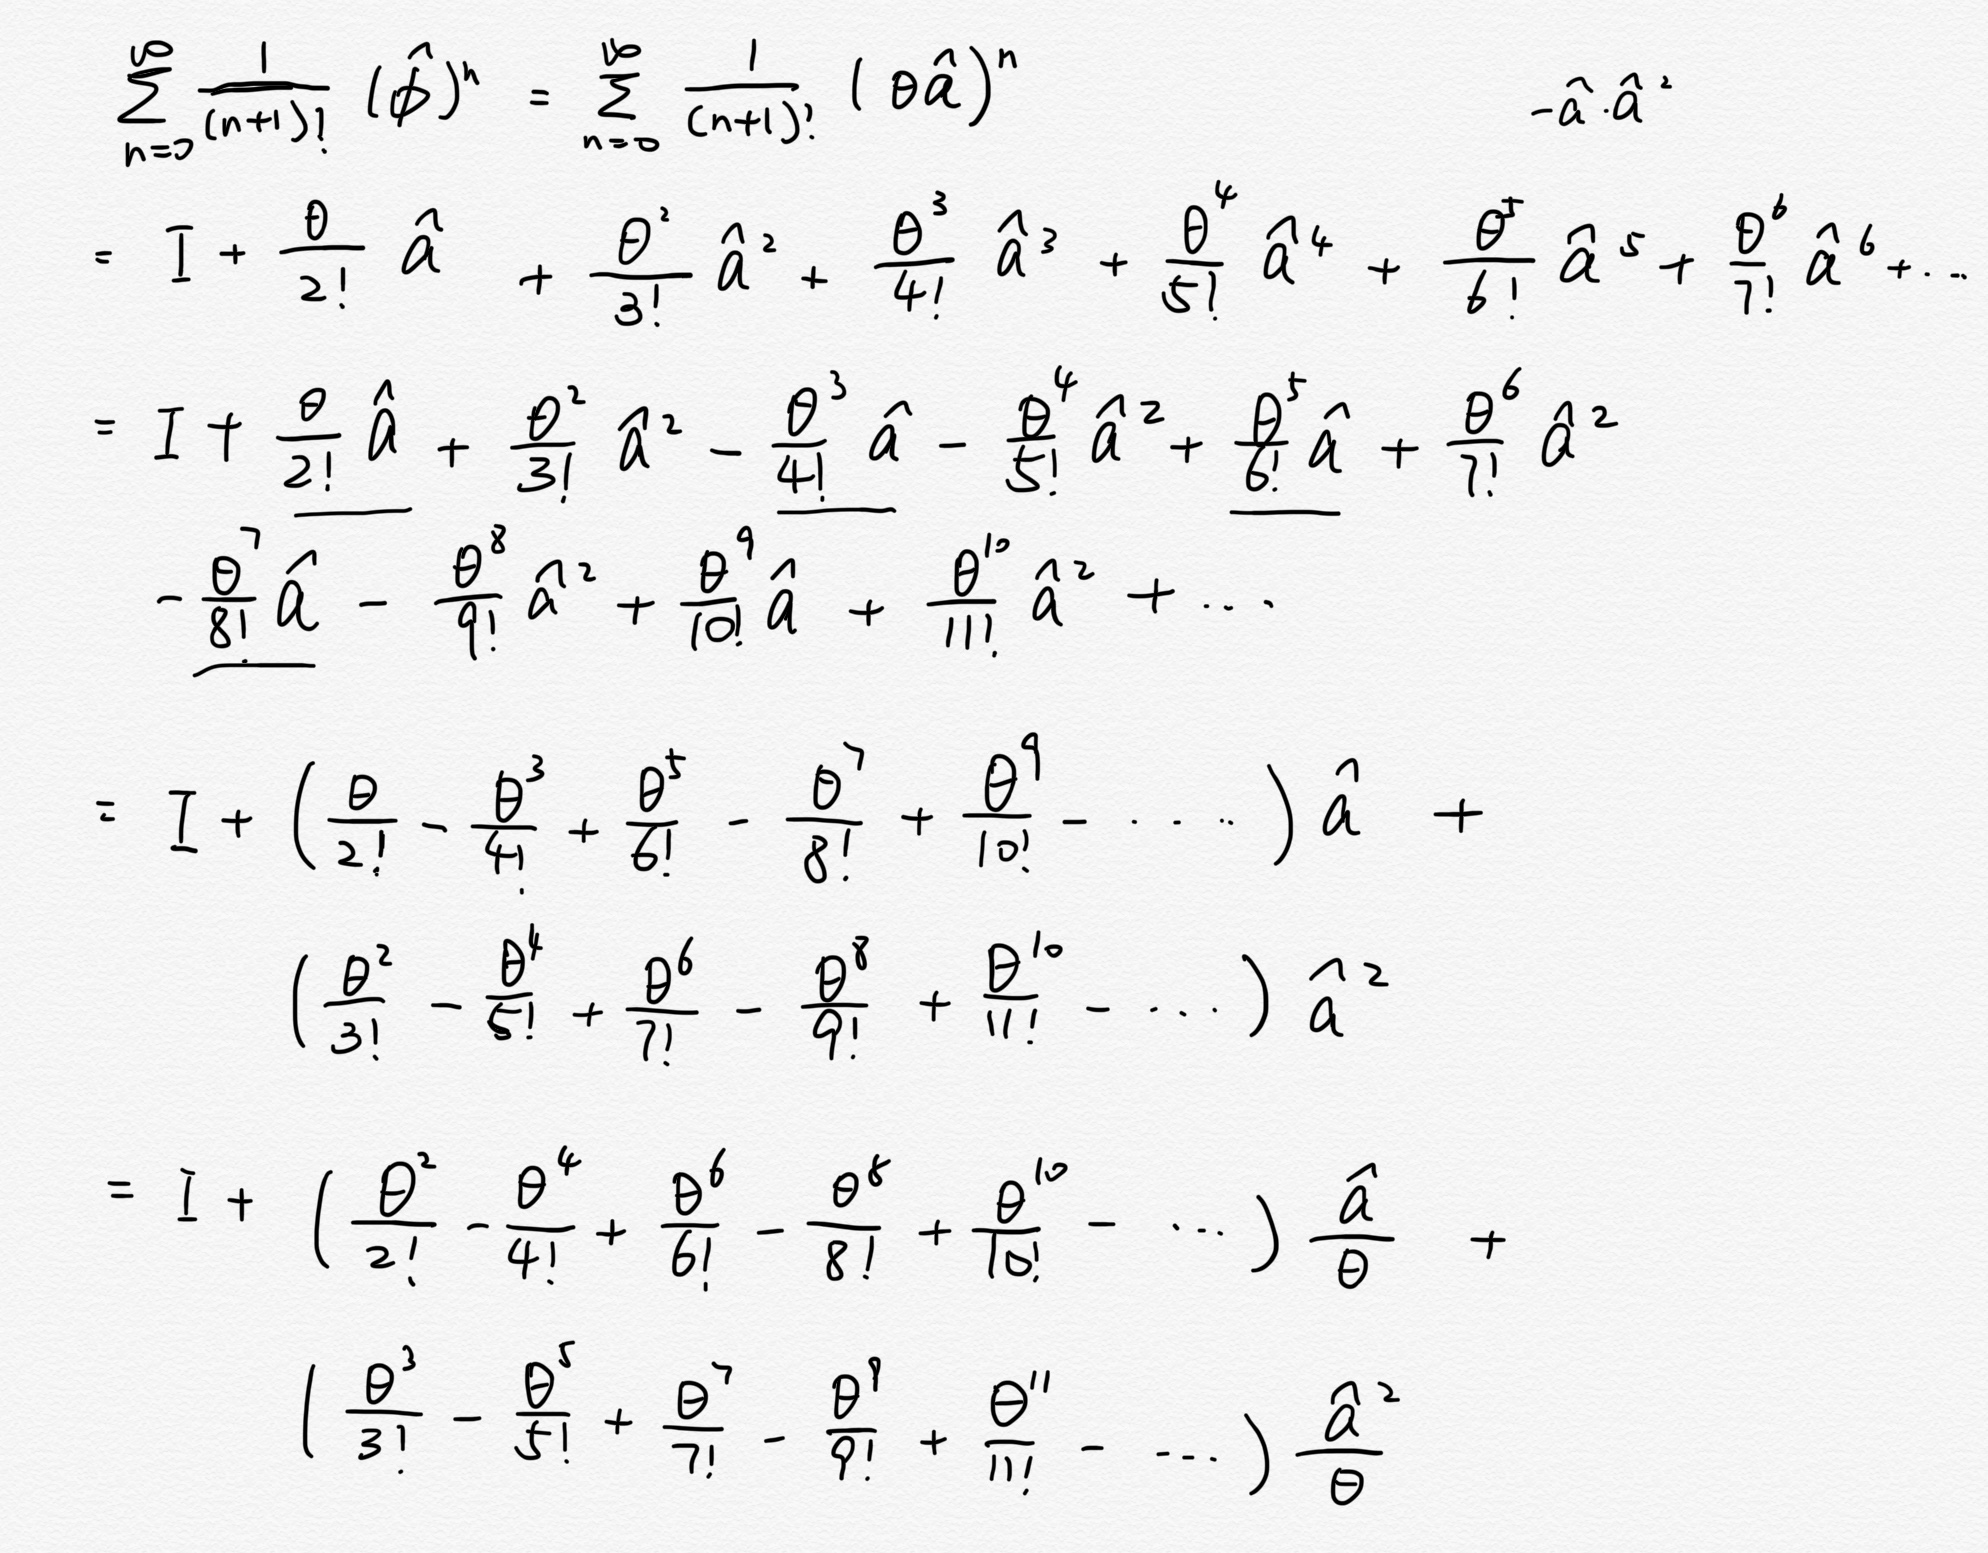
\includegraphics[width=\textwidth]{images/eq1.png}
  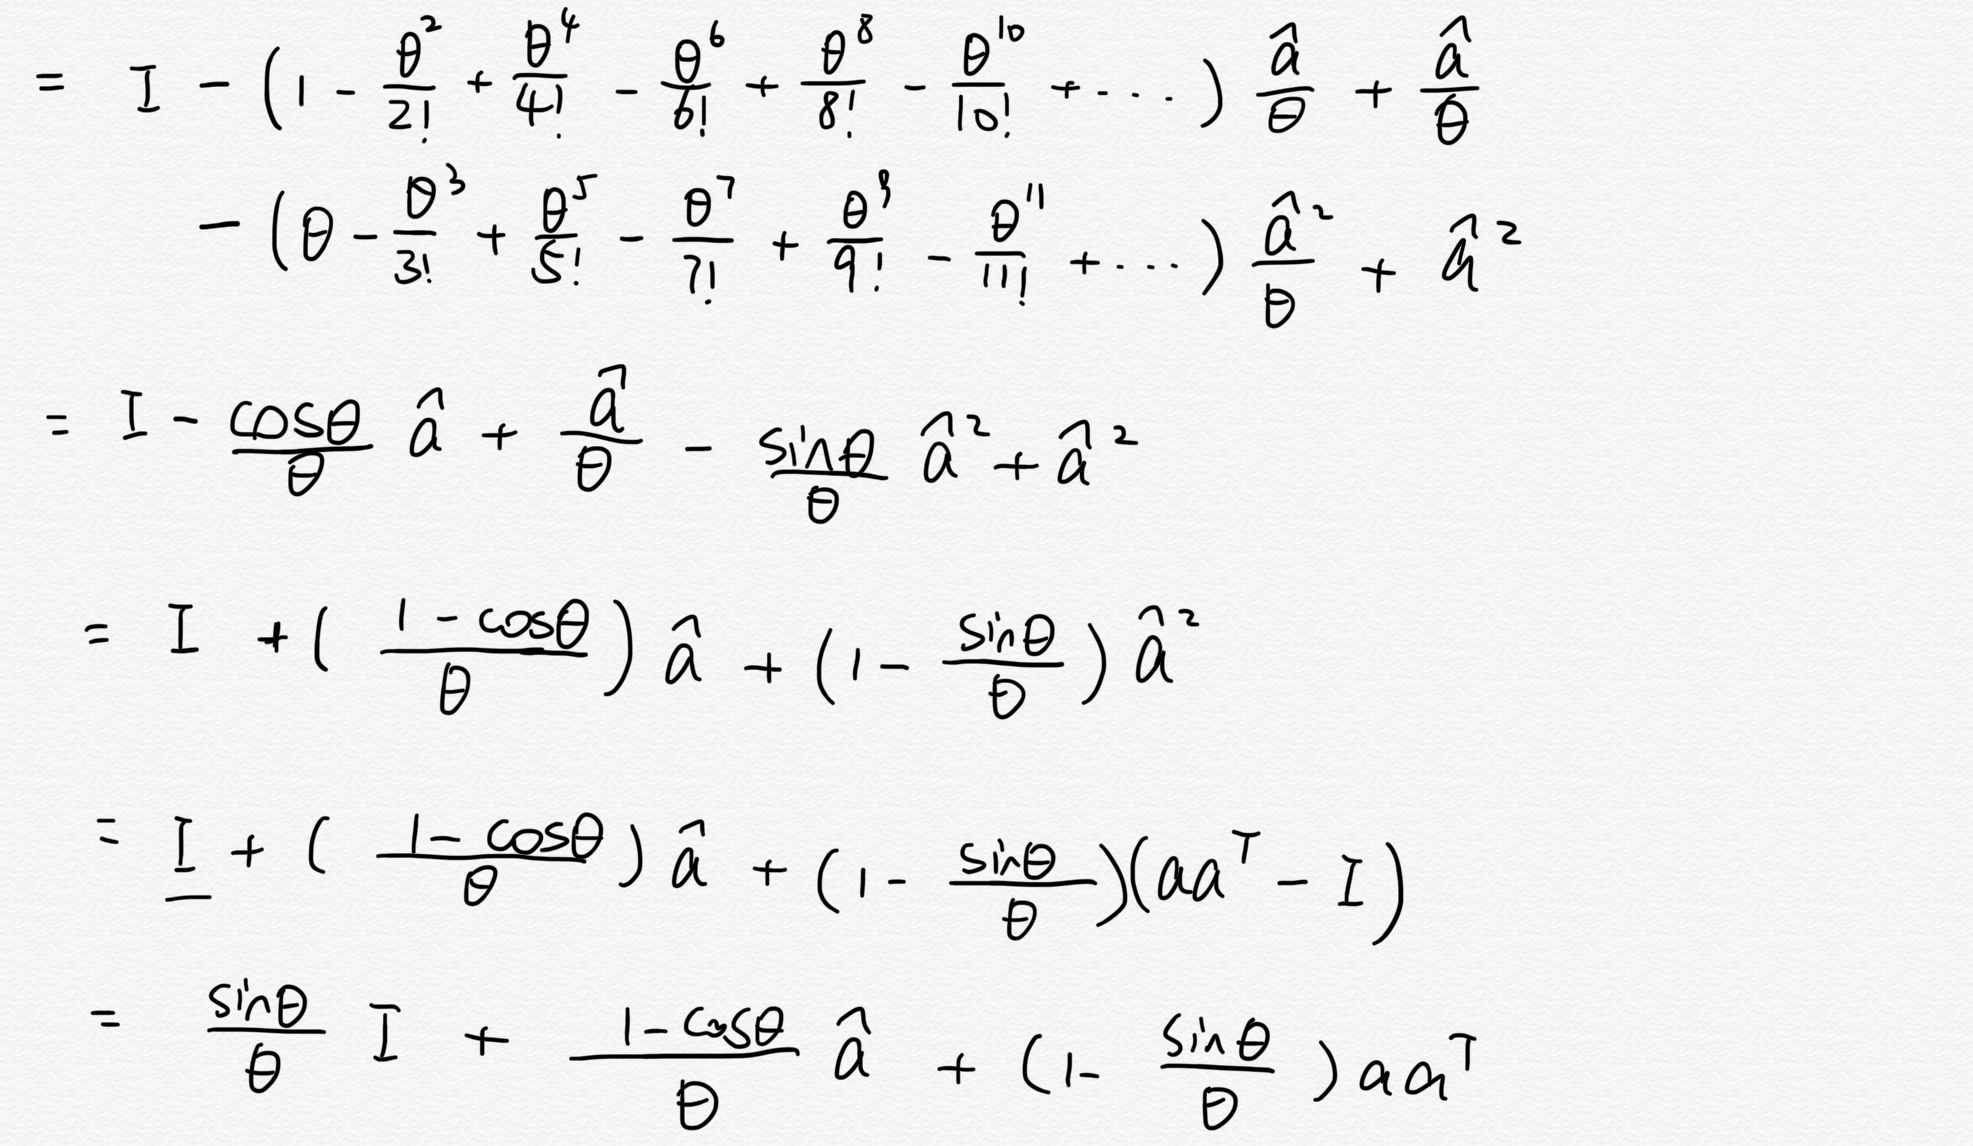
\includegraphics[width=\textwidth]{images/eq2.png}
  \caption{Prove of the equation 2}
\end{figure}


%---------------------------------------------------------------------------
\end{document}